\documentclass[11pt, a4paper]{article}

\usepackage{style}

\institution{EPFL}
\project{Semester Project}
\title{Minimal Rational Interpolation for Time-Harmonic Maxwell's Equations}
\author{Fabio Matti}
\supervisor{Prof. Fabio Nobile \\ Dr. Davide Pradovera}
\date{\today}

\begin{document}

\maketitle

\section*{Abstract}
\label{sec:abstract}

\pagebreak
\tableofcontents

\pagebreak
\section{Introduction}
\label{sec:introduction}

\pagebreak
\section{Finite element discretization of the time-harmonic Maxwell's equations}
\label{sec:maxwell}

\subsection{Vector potential formulation of the time-harmonic Maxwell's equations}
\label{subsec:maxwell-potential}

% Everything smooth enough to do all manipulations...

Let $\mathbf{E}$ denote an electric field, $\mathbf{B}$ a magnetic field
strength, $\rho$ an electric charge density, and $\mathbf{j}$ an electric
current density. Maxwell's equations are stated in \citep{monk} as
\begin{align}
    \nabla \cdot (\epsilon \mathbf{E}) &= \rho \label{equ:maxwell1} \\
    \nabla \cdot \mathbf{B} &= 0 \label{equ:maxwell2} \\
    \nabla \times \mathbf{E} &= -\partial_t \mathbf{B} \label{equ:maxwell3} \\
    \nabla \times (\mu^{-1} \mathbf{B}) &= \partial_t (\epsilon \mathbf{E}) + \mathbf{j} \label{equ:maxwell4}
\end{align}
with $\varepsilon$ being the permittivity and $\mu$ the permeability.

% Non-conducting material, else => j = sigma*E + J_a (Monk 21)

Equation (\ref{equ:maxwell2}) allows for an expression of the magnetic field 
$\mathbf{B} = \nabla \times \mathbf{u}$ in terms of a vector valued function
$\mathbf{u}$, the vector potential (in literature commonly denoted with
$\mathbf{A}$). Similarly, (\ref{equ:maxwell3}) suggests
rewriting the electric field $\mathbf{E} = - \nabla \phi - \partial_t \mathbf{u}$
using a scalar function $\phi$, referred to as the scalar potential.

The physical quantities $\mathbf{E}$ and $\mathbf{B}$ remain unchanged 
if we transform $\mathbf{u} \to \mathbf{u}' = \mathbf{u} + \nabla \psi$ or
$\phi \to \phi' = \phi - \partial_t \psi$ for arbitrary functions $\psi$.
A convenient choice of $\psi$ is suggested in \citep{gauge-transformation} to be
\begin{equation}
    \psi = \int_0^t \phi dt' \label{equ:gauge}
\end{equation}
which transforms $\phi \to \phi' = 0$ and $\mathbf{u} \to \mathbf{u}' = \mathbf{u}
+ \nabla \int_0^t \phi dt'$. Thus, the expressions for the electrical and
magnetic field become
\begin{align}
    \mathbf{E} &= -\partial_t \mathbf{u} \label{equ:electricfield} \\
    \mathbf{B} &= \nabla \times \mathbf{u} \label{equ:magneticfield}
\end{align}
where I renamed the variable $\mathbf{u}'$ to $\mathbf{u}$ for simplicity.

Plugging the identities (\ref{equ:electricfield}) and (\ref{equ:magneticfield})
into (\ref{equ:maxwell4}) yields 
\begin{equation}
    \nabla \times (\mu^{-1} \nabla \times \mathbf{u}) =  \epsilon \partial_t^2 \mathbf{u} + \mathbf{j} \label{equ:maxwell-potential}
\end{equation}

For the rest of this report, I restrict myself to vector potentials $\mathbf{u}$
that exhibit a harmonic dependence on time $t$, i.e. may be factorized into
a term solely depending on the position $\mathbf{x}$ and a complex exponential
\begin{equation}
    \mathbf{u}(\mathbf{x}, t) = \mathbf{u}(\mathbf{x}) \exp(i \omega t) \label{equ:time-harmonic}
\end{equation}
Substituting this expression into (\ref{equ:maxwell-potential}) results in the
\begin{fancybox}{Time-harmonic potential equation}
    \begin{equation}
     \nabla \times (\mu^{-1} \nabla \times \mathbf{u}) - \epsilon \omega^2 \mathbf{u} = \mathbf{j} \label{equ:maxwell-timeharmonic}
    \end{equation}
\end{fancybox}

\subsection{Weak formulation for the time-harmonic potential equation}
\label{subsec:maxwell-weak}

Equation (\ref{equ:maxwell-timeharmonic}) may be multiplied by a vector-valued
function $\mathbf{v} \in H_{\textrm{curl}}(\Omega)$, where
\begin{equation}
    H_{\textrm{curl}}(\Omega) = \{\mathbf{u} : \Omega \to \mathbb{C},~\text{such that}~\mathbf{u}\in L^2(\mathbb{C})^3, \nabla \times \mathbf{u} \in L^2(\mathbb{C})^3\} \label{equ:h-curl}
\end{equation}
and then integrated over all of $\Omega$ to obtain 
\begin{equation}
    \int_{\Omega} (\nabla \times ({\mu^{-1} \nabla \times \mathbf{u}})) \cdot \mathbf{v}
    - \omega^2 \int_{\Omega} \epsilon \mathbf{u} \cdot \mathbf{v} = \int_{\Omega} \mathbf{j} \cdot \mathbf{v} \label{equ:maxwell-weak-initial}
\end{equation}
% !REMINDME: Put derivation in appendix
This may further be simplified (\ref{equ:maxwell-weak-initial}) to (see Section 
\ref{sec:abstract} for details)
\begin{fancybox}{Weak formulation of the time-harmonic potential equation}
    \begin{equation}
        \int_{\Omega} ({\mu^{-1} \nabla \times \mathbf{u}}) \cdot (\nabla \times \mathbf{v})
        - \omega^2 \int_{\Omega} \epsilon \mathbf{u} \cdot \mathbf{v} 
        = \int_{\Omega} \mathbf{j} \cdot \mathbf{v}
        + \int_{\partial \Omega} \underbrace{(({\mu^{-1} \nabla \times \mathbf{u}}) \times \mathbf{n})}_{= \mathbf{g}} \cdot \mathbf{v}
        \label{equ:maxwell-weak}
    \end{equation}
\end{fancybox}
where $\mathbf{n}$ denotes the surface normal to the boundary $\partial \Omega$.

Boundary conditions on the electric field $\mathbf{E}$ may be enforced in a Dirichlet-type
fashion through the relation (\ref{equ:electricfield}) and the assumption
(\ref{equ:time-harmonic})
\begin{equation}
    \left.\mathbf{u}\right|_{\partial \Omega} = -\frac{1}{i\omega} \left.\mathbf{E}\right|_{\partial \Omega} \label{equ:dirichlet-boundary}
\end{equation}
Those on the magnetic field $\mathbf{B}$ through a Neumann-type condition following
from (\ref{equ:magneticfield}) and again (\ref{equ:time-harmonic})
\begin{equation}
    \left.\mathbf{g}\right|_{\partial \Omega} = (\mu^{-1} \left.\mathbf{B}\right|_{\partial \Omega}) \times \mathbf{n} \label{equ:neumann-boundary}
\end{equation}

\subsection{Two-dimensional resonant cavity}
\label{subsec:cavity}

A resonant cavity is a region $\Omega$ enclosed by a boundary $\partial \Omega$.
The boundary is subdivided into one (or more) inlets $\Gamma_N$ and a perfect
electrically conducting wall $\Gamma_D = \partial \Omega \setminus \Gamma_N$.

\begin{figure}[h]
    \centering
    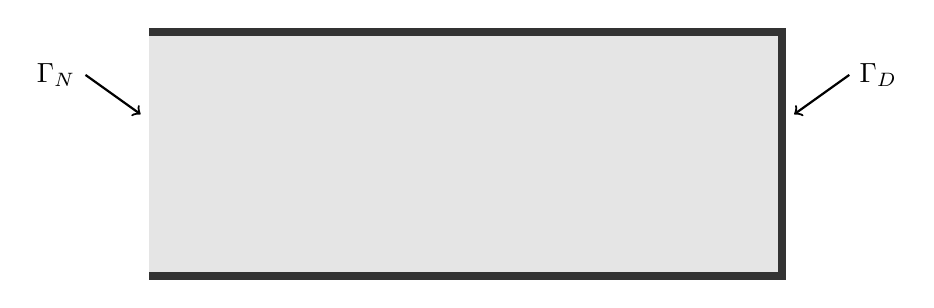
\begin{tikzpicture}
    \fill[black!80!white] (0, -0.1) rectangle (8.1, 3.1);
    \fill[black!10!white] (0, 0) rectangle (8, 3);
    \draw[thick, ->] (-0.8, 2.5) node[left] {$\Gamma_N$} to (-0.1, 2);
    \draw[thick, ->] (8.9, 2.5) node[right] {$\Gamma_D$} to (8.2, 2);
\end{tikzpicture}
    \caption{Example of a two-dimensional resonant cavity: The rectangular
    cavity.}
    \label{fig:2d-waveguide}
\end{figure}

% !REMINDME: Why only need test against v_z?!
Suppose the current density $\mathbf{j} \equiv 0$ and orient the coordinate
system in such a way that $\mathbf{u} = u_z \mathbf{e}_z$ and 
$\mathbf{v} = v_z \mathbf{e}_z$. Consequently,
\begin{equation}
    (\mu^{-1} \nabla \times \mathbf{u}) \cdot (\nabla \times \mathbf{v})
    = (\mu^{-1} \nabla u_z) \cdot (\nabla v_z)
\end{equation}
Use $g_z = (\mathbf{g})_z$ along the boundary $\Gamma_N$,
to convert (\ref{equ:maxwell-weak}) into
the weak formulation for a two-dimensional resonant cavity
\begin{equation}
    \int_{\Omega} (\mu^{-1} \nabla u_z) \cdot (\nabla v_z)
    - \omega^2 \int_{\Omega} \epsilon u_z v_z
    = \int_{\partial \Omega} g_z v_z \label{equ:maxwell-weak-resonant-cavity}
\end{equation}

% Boundary conditions Dirichlet and Neumann (from Monk)
Let $\mathbf{E}$ and $\mathbf{B}$ refer to the electric and magnetic fields inside
the cavity. For now, I distinguish two types of boundaries.

For the perfectly conducting boundary, treated in \citep{monk}, it holds that
\begin{equation}
    \mathbf{n} \times \mathbf{E} = 0,~~\text{on}~\Gamma_D
\end{equation}
For the boundaries in a two-dimensional resonant cavity (see Figure 
\ref{fig:2d-waveguide}), this only holds true if $E_z = 0$, which translates
to the Dirichlet boundary condition $\left.\mathbf{u}\right|_{\Gamma_D} = 0$
in light of (\ref{equ:dirichlet-boundary}).

For the inlet, it is easiest to enforce the boundary condition through the
magnetic field $\mathbf{B}$ (considering $\mathbf{n} = -\mathbf{e}_x$ as
depicted in Figure \ref{fig:2d-waveguide}):
\begin{equation}
    g_z = (({\mu^{-1} \mathbf{B}}) \times (-\mathbf{e}_x))_z = \mu^{-1} B_x
\end{equation}



\subsection{Waveguide}
\label{subsec:waveguide}

% Just j=0 and 3d, need to discuss boundary conditions

\subsection{Imperfect conductor}
\label{subsec:impedance}

% Additionally impedance boundary condition from Monk

%%% Maybe need a chapter on finite element approximation + description of usage
% of fenics or such

\pagebreak
\section{Finite element approximation with FEniCS}
\label{sec:fem}

% Theory (Galerkin and such)

$a_{\omega}(u, v) = L(v)$.

% Demonstration

% Nédelec elements

\pagebreak
\section{Greedy minimal rational interpolation for the time-harmonic Maxwell's equations}
\label{sec:mri}

% General idea 


% Algorithm (last column SVD is definition of MRI, cite Davide)
\citep{greedyMRI}

\begin{algorithm}
    \caption{Minimal rational interpolation} \label{alg:MRI}
    \begin{algorithmic}
    \Require $\omega_1, \dots, \omega_S$
    \Require $U = [u(\omega_1) | \dots | u(\omega_S)]$ \Comment{Snapshot matrix}
    \State Compute $G$ with $g_{ij} = \langle u(\omega_i), u(\omega_j)\rangle_M,~ i, j \in \{1, \dots, S \}$ \Comment{Gramian matrix}
    \State Compute the singular value decomposition $G = V \Sigma V^H$
    \State Define $q = V[:, S]$
    \State Define $\tilde{u}(\omega) = P(\omega) / Q(\omega)$ with $P(\omega) = \sum_{j=1}^S \frac{q_j u(\omega_j)}{\omega - \omega_j}$ and $Q(\omega) = \sum_{j=1}^S \frac{q_j}{\omega - \omega_j}$
\end{algorithmic}
\end{algorithm}

\citep{shortMRI}

\begin{algorithm}
    \caption{Greedy minimal rational interpolation} \label{alg:gMRI}
    \begin{algorithmic}
    \Require $\tau > 0$ \Comment{Relative $L_2$-error tolerance}
    \Require $\Omega_{\mathrm{test}} = \{\omega_i\}_{i=1}^M$ \Comment{Set of candidate support points}
    \Require $a_{\omega}(\mathbf{u}, \mathbf{v}) = L(\mathbf{v})$ \Comment{Finite element formulation of the problem}
    \State Choose $\omega_1, \dots, \omega_t \in \Omega_{\mathrm{test}}$ \Comment{Usually the smallest and largest element}
    \State Remove $\omega_1, \dots, \omega_t$ from $\Omega_{\mathrm{test}}$
    \State Solve $a_{\omega_i}(\mathbf{u}_i, \mathbf{v}) = L(\mathbf{v})$ for $i \in \{1, \dots, t\}$
    \State Build surrogate $\mathbf{\tilde{u}}_t = \mathbf{P}_t(\omega) / Q_t(\omega)$ using the solutions $\mathbf{u}_1, \dots, \mathbf{u}_t$
    \While{$\Omega_{\mathrm{test}} \neq \emptyset$}
        \State $\omega_{t+1} \leftarrow \textrm{argmin}_{\omega \in \Omega_{\mathrm{test}}} |Q_t(\omega)|$
        \State Solve $a_{\omega_{t+1}}(\mathbf{u}_{t+1}, \mathbf{v}) = L(\mathbf{v})$
        \State Build surrogate $\mathbf{\tilde{u}}_{t+1} = \mathbf{P}_{t+1}(\omega) / Q_{t+1}(\omega)$ using the solutions $\mathbf{u}_1, \dots, \mathbf{u}_{t+1}$
        \If{$||\mathbf{u}_{t+1} - \mathbf{\tilde{u}}_{t}(\omega_{t+1})||_M / ||\mathbf{u}_{t+1}||_M < \tau$}
            \Return
        \EndIf
        \State $t \leftarrow t+1$
    \EndWhile
    %\Return $\tilde{A}(\omega) = \sum_i \frac{q_i A(\omega_i)}{\omega - \omega_i} / \sum_i \frac{q_i}{\omega - \omega_i}$
\end{algorithmic}
\end{algorithm}

% Interpolation property (in barycentric expansion, l'Hôpital whatever)

% Rational root finding 

\citep{klein}

Defining 
\begin{equation}
    v_i = (\omega - \omega_i)^{-1}
\end{equation}
and requiring
\begin{equation}
    0 = Q(\omega) = \sum_{i=1}^S q_i v_i(\omega)
\end{equation}
can be equivalently expressed as a generalized eigenvalue problem
\begin{equation}
    \mathbf{\underline{A}} \mathbf{u} = \omega \mathbf{\underline{B}} \mathbf{u}
\end{equation}
with
\begin{equation}
    \mathbf{\underline{A}} = \begin{pmatrix}
        0 & q_1 & q_2 & \dots & q_S \\
        1 & \omega_1 & & & \\
        1 & & \omega_2 & & \\ 
        \vdots & & & \ddots & \\ 
        1 & & & & \omega_S
    \end{pmatrix} ~~\text{and}~~ 
    \mathbf{\underline{B}} = \begin{pmatrix}
        0 & & & & \\
         & 1 & & & \\
         & & 1 & & \\ 
        \vdots & & & \ddots & \\ 
         & & & & 1
    \end{pmatrix}\label{equ:root-finding}
\end{equation}

% Optimization tweaks

% -> Householder sequential algorithm instead of full Gramian

\citep{householder}

\begin{algorithm}
    \caption{Additive Householder triangularization} \label{alg:householder}
    \begin{algorithmic}
\Require $U[1 \dots s, 1 \dots N]$ \Comment{Next snapshot matrix}
\Require $R[1 \dots S, 1 \dots S]$  \Comment{Previous triangular matrix}
\Require $E[1 \dots S, 1 \dots N]$ \Comment{Previous orthonormal matrix}
\Require $V[1 \dots S, 1 \dots N]$ \Comment{Previous Householder matrix}
\State Extend size of $R$ to $(S + s) \times (S + s)$
\State Extend $E$ with $S$ orthonormal columns to $(S + s) \times N$
\State Extend size of $V$ to $(S + s) \times N$
\For{$j = S+1:S+s$}
    \State $u = U[j]$
    \For{$k = 1:j-1$}
        \State $u \leftarrow u - 2 \langle V[k, :], u \rangle_M V[k, :]$
        \State $R[k, j] \leftarrow \langle E[k, :], u \rangle_M$
        \State $u \leftarrow u - R[k, j] E[k, :]$
    \EndFor
    \State $R[j, j] \leftarrow ||u||_M$
    \State $\alpha \leftarrow \langle E[j, :], u \rangle_M$
    \If{$|\alpha| \neq 0$}
        \State $E[j, :] \leftarrow E[j, :] (-\alpha / |\alpha|)$
    \EndIf 
    \State $V[j, :] \leftarrow R[j, j] E[j, :] - u$
    \State $V[j, :] \leftarrow V[j, :] - \langle E[S+1:j], V[j, :] \rangle_M E[S+1:j, :]$
    \State $\sigma \leftarrow ||V[j, :]||_M$
    \If{$\sigma \neq 0$}
        \State $V[j, :] \leftarrow V[j, :] / \sigma$
    \Else
        \State$V[j, :] \leftarrow E[j, :]$
    \EndIf
\EndFor
\end{algorithmic}
\end{algorithm}

% -> Check stability of build with SVDs

% -> Model order reduction techniques (u_ring, error computation, ...)

\pagebreak
\section{Examples}
\label{sec:examples}

\subsection{Two-dimensional rectangular cavity}
\label{subsec:examples-rectangularcavity}

% Exploratory plots

% Rational interpolation demonstration

% Analytical root finding

% Problems with non-resonant solutions suppressed by the boundary integral

% Problems with linearly combinable solutions -> Use cubby to perturb waveguide

\subsection{Dual mode circular waveguide filter}
\label{subsec:examples-dmcwf}

% Describe geometry and physical meaning

\begin{figure}[h]
    \centering
    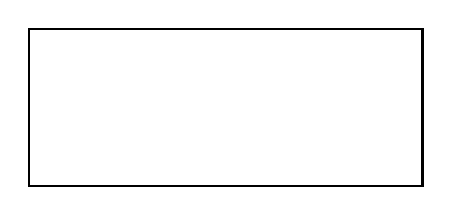
\begin{tikzpicture}
    \draw[thick] (0, 0) rectangle (5, 2);
\end{tikzpicture}
    \caption{Dual-mode circular waveguide filter.}
    \label{fig:DMCWF}
\end{figure}

% Modeling process cite rubia

% Scattering coefficient

% Measurement procedure

\subsection{Imperfectly conducting boundaries}
\label{subsec:examples-impedance}

% Pole plot

\pagebreak
\section{Conclusion and outlook}
\label{sec:conclusion}

% Danksagung

\pagebreak
\section{Appendix}
\label{sec:appendix}

\subsection{Detailed derivation for the weak formulation of the time-harmonic potential equation}
\label{subsec:derivation}

% !REMINDME: Levi-Civita tensor explanations.
The goal is to rewrite the curl-integral on the left-hand side of 
(\ref{equ:maxwell-weak-initial}):
\begin{equation}
    \int_{\Omega} (\nabla \times (\mu^{-1} \nabla \times \mathbf{u})) \cdot \mathbf{v} \label{equ:maxwell-weak-initial-LHS}
\end{equation}
In order to simplify the curls and apply the Gauss theorem, I first show
the following vector calculus identity:
\begin{fancybox}{Curl product rule}
    \begin{equation}
        (\nabla \times \mathbf{a}) \cdot \mathbf{b} = \nabla \cdot (\mathbf{a} \times \mathbf{b}) + \mathbf{a} \cdot (\nabla \times \mathbf{b}) \label{equ:vector-calculus} \\
    \end{equation}
\end{fancybox}
% !REMINDME: Appropriate spaces
where $\mathbf{a}$, $\mathbf{b}$ are vector-value functions. The completely
antisymmetric tensor $\varepsilon_{ijk}$, frequently referred to as the
Levi-Civita tensor, may be employed to rewrite the components of the
curl of a vector-function $\mathbf{a}$ as the sum
% !REMINDME: Maybe lemma and proof formatting
\begin{equation}
    (\nabla \times \mathbf{a})_k = \sum_i \sum_j \varepsilon_{ijk} \partial_i u_j
\end{equation}
where $\partial_i$ denotes the partial derivative with respect to the $i$-th coordinate
direction. This yields
\begin{align}
    (\nabla \times \mathbf{a}) \cdot \mathbf{b} &= \sum_k (\nabla \times \mathbf{a})_k b_k \notag \\ 
    &= \sum_k (\sum_i \sum_j \varepsilon_{ijk} \partial_i a_j) b_k \notag \\ 
    &= \sum_k \sum_i \sum_j \partial_i (\varepsilon_{ijk} a_j b_k) - \sum_k \sum_i \sum_j a_j (\varepsilon_{ijk} \partial_i b_k) \notag \\ 
    &= \sum_k \sum_i \sum_j \partial_i (\varepsilon_{jki} a_j b_k) - \sum_k \sum_i \sum_j a_j ((-\varepsilon_{ikj}) \partial_i b_k) \notag \\ 
    &= \sum_i \partial_i (\mathbf{a} \times \mathbf{b})_i + \sum_j u_j (\nabla \times \mathbf{b})_j \notag \\ 
    &= \nabla \cdot (\mathbf{a} \times \mathbf{b}) + \mathbf{a} \cdot (\nabla \times \mathbf{b}) \label{equ:curlidentity} 
\end{align}
by expressing the scalar product as a component-sum, using the product rule and
applying the symmetry and anti-symmetry properties of the Levi-Civita tensor.
Now the identity (\ref{equ:vector-calculus}) to (\ref{equ:maxwell-weak-initial-LHS})
together with Gauss' theorem gives
\begin{align}
    \int_{\Omega} (\nabla \times ({\mu^{-1} \nabla \times \mathbf{u}})) \cdot \mathbf{v} &=
    \int_{\Omega} \nabla \cdot (({\mu^{-1} \nabla \times \mathbf{u}}) \times \mathbf{v})
    + \int_{\Omega} ({\mu^{-1} \nabla \times \mathbf{u}}) \cdot (\nabla \times \mathbf{v}) \notag \\
    &= \int_{\partial \Omega} (({\mu^{-1} \nabla \times \mathbf{u}}) \times \mathbf{v}) \cdot \mathbf{n}
    + \int_{\Omega} ({\mu^{-1} \nabla \times \mathbf{u}}) \cdot (\nabla \times \mathbf{v}) \notag \\
\end{align}

For later convenience, the boundary integral can further be simplified using the
\begin{fancybox}{Commutative behavior of the scalar triple product}
    \begin{equation}
        (\mathbf{a} \times \mathbf{b}) \cdot \mathbf{c} = - (\mathbf{a} \times \mathbf{c}) \cdot \mathbf{b} \label{equ:vector-algebra}
    \end{equation}
\end{fancybox}
This identity follows immediately from a small manipulation with the Levi-Civita
tensor:
\begin{align}
    (\mathbf{a} \times \mathbf{b}) \cdot \mathbf{c} &= \sum_k (\sum_i \sum_j \varepsilon_{ijk} a_i b_j) c_k \notag \\
     &= \sum_j (\sum_i \sum_k (-\varepsilon_{ikj}) a_i c_k) b_j \notag \\ 
     &= - (\mathbf{a} \times \mathbf{c}) \cdot \mathbf{b} 
\end{align}
The boundary integral becomes 
\begin{equation}
    \int_{\partial \Omega} (({\mu^{-1} \nabla \times \mathbf{u}}) \times \mathbf{v}) \cdot \mathbf{n}
    = - \int_{\partial \Omega} (({\mu^{-1} \nabla \times \mathbf{u}}) \times \mathbf{n}) \cdot \mathbf{v}
\end{equation}

This concludes the short derivation, because now (\ref{equ:maxwell-weak-initial-LHS})
may be rewritten as
\begin{equation}
    - \int_{\partial \Omega} (({\mu^{-1} \nabla \times \mathbf{u}}) \times \mathbf{v}) \cdot \mathbf{n}
    + \int_{\Omega} ({\mu^{-1} \nabla \times \mathbf{u}}) \cdot (\nabla \times \mathbf{v})
\end{equation}

% 
\newpage
\bibliography{biblio.bib}

\end{document}